%****************************************************
%	CHAPTER 2 - Prototype Design
%****************************************************
\chapter{Prototype Design}
\label{ch:proto}
%====================================================
\section{Conventions Used}
\label{sec:proto.conventions}
The attitude conventions used for the systems' dynamic derivations in the following Chapter:\ref{ch:dynamics} are first briefly discussed here. Often these aspects are omitted or assumed to be known already. It's important to clearly and unambiguously define a standard set of framing conventions to avoid uncertainty later. Rotation matrices are included but the focus remains on the \emph{contrast} between a rotation and transformation operation. Both \cite{spacecraftattitutdequaternions} and \cite{rigidbodylecture} provide an in depth and thorough explanation of rotation matrices and DCM attitude representation if such concepts are unfamiliar to the reader.
%====================================================
\subsection{Reference Frames Convention}
\label{subsec:proto.conventions.frames}
%====================================================
\begin{figure}[htbp]
\centering
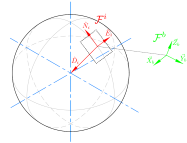
\includegraphics[width=0.6\textwidth]{figs/reference_frame}
\caption{Inertial and Body Reference Frames}
\label{fig:ref_frame}
\end{figure}
Euler (aerospace) frames are used for principle inertial and body coordinates (Fig:\ref{fig:ref_frame}). The inertial frame,~$\mathcal{F}^i$, is aligned such that the $\vec{X}_i$ axis is in the $\hat{N}$orth direction, $\vec{Y}_i$ is in the $\hat{E}$ast direction and $\vec{Z}_i$ is  in the $\hat{D}$ownward direction\footnote{In orbital sequences this would be toward the Earths' center. Sometimes referred to as the NED convention}. The body frame, $\mathcal{F}^b$, then has both $\vec{X}_b$ and $\vec{Y}_b$ aligned with two perpendicular arms of the quadrotors' body and the $\vec{Z}_b$ axis in the body's normal direction (Fig:\ref{fig:body-frame}). The body frames' axes and their relation to the prototype design are highlighted next in Section:\ref{subsec:proto.conventions.motoraxis}. Frame superscripts $i$ and $b$ represent inertial and body frames respectively whilst vector subscripts imply the reference frame in which the vectors' coordinates exists in.
\par
Relative angular displacement between two frames is commonly measured by the three angle Euler set. The Euler angles $\Upsilon=[\phi ~\theta ~\psi]^T$ represents rotations about the $\vec{X}$,$\vec{Y}$ and $\vec{Z}$ axes respectively. Depending on how the rotation sequence is formulated, those angles can be used to construct rotation matrices which give relation to vectors or can transform coordinates. The generic equation to rotate a vector $\vec{v}$ about a (normalized) axis $\hat{n}$ by some angle $\mu$ is given by\footnote{Derived and proven in \emph{Quadrotor Dynamics and Control}\cite{quaddynamics}}:
\begin{equation}\label{eq:genrotationmatrix}
\vec{v}~'=\big(1-cos(\mu)\big)\big(\vec{v}\cdot \hat{n}\big)\hat{n}+cos(\mu)\vec{v}+sin(\mu)\big(\hat{n}\times\vec{v}\big)
\end{equation}
Which, when $\hat{n}$ is either $\vec{X}$,$\vec{Y}$ or $\vec{Z}$ axes, can be simplified to produce the common rotation matrices $\mathbb{R}_x(\phi)$,$\mathbb{R}_y(\theta)$ and $\mathbb{R}_z(\psi)$. Multiplication by a rotation matrix $\mathbb{R}(\cdot)$ applies a left-handed \emph{rotation} operator, the resultant vector still exists in the same reference frame;
\begin{subequations} \label{eq:rotationoperator}
\begin{equation}\label{eq:rotationoperator.a}
\vec{v}~'=\mathbb{R}_{x}(\phi)\vec{v}
\end{equation}
\vspace{-20pt}
\begin{equation}\label{eq:rotationoperator.b}
\vec{v}~',\vec{v}\in\mathcal{F}^1
\end{equation}
\end{subequations}
\emph{\color{Gray} No subscripts are used in Eq: \ref{eq:rotationoperator} to indicate reference frame ownership because all vectors are in the same frame}
\par
A \emph{transformation} changes the vectors reference frame. The transformation is a rotation by an angle of the difference between the resulting and principle reference frames. A transformation from frame $\mathcal{F}^1$ to $\mathcal{F}^2$, differing by an angle of $\phi$ about the $\vec{X}$ axis is then:
\begin{subequations}\label{eq:transformationoperator}
\begin{equation}\label{eq:transformationoperator.a}
\vec{v}_2=\mathbb{R}_x(-\phi)\vec{v}_1
\end{equation}
\vspace{-20pt}
\begin{equation}\label{eq:transformationoperator.b}
\vec{v}_2\in\mathcal{F}^2~\text{and}~\vec{v}_1\in\mathcal{F}^1
\end{equation}
\end{subequations}
The distinction between Eq:\ref{eq:rotationoperator} and Eq:\ref{eq:transformationoperator} is the sense of the angular operand $\phi$, and hence the effect it has on the argument vector. The transformation of a vector from $\mathcal{F}^i$ to $\mathcal{F}^b$ is the product of three sequential operations about each of the axes. Because each subsequent rotation is applied relative to a new  intermediate frame, the sequence of axial rotations will effect the Euler set. Any consequences of that chosen order is something well documented in \emph{Quaternions and Rotation Sequence}, \cite{rotationsequences}. In this dissertation the ZYX sequence is used. Hence a transformation of a vector $\vec{v}$ from the inertial to the body frame is applied by:
\begin{subequations}
\begin{equation}\label{eq:inertialbodytransformation.a}
\mathbb{R}_{i}^{b}\triangleq\mathbb{R}_z(\psi)\mathbb{R}_y(\theta)\mathbb{R}_x(\phi)
\end{equation}
\vspace{-15pt}
\begin{equation}\label{eq:inertialbodytransformation.b}
\vec{v}_b=\mathbb{R}_i^b(-\psi,-\theta,-\phi)\vec{v}_i
\end{equation}
\vspace{-15pt}
\begin{equation}\label{eq:inertialbodytransformation.c}
\Rightarrow\vec{v}_b=\mathbb{R}_z(-\psi)\mathbb{R}_y(-\theta)\mathbb{R}_x(-\phi)\vec{v}_i
\end{equation}
\vspace{-15pt}
\begin{equation} \label{eq:inertialbodytransformation.d}
\mathbb{R}_z(-\psi)\mathbb{R}_y(-\theta)\mathbb{R}_x(-\phi) \iff \mathbb{R}_x(\phi)\mathbb{R}_y(\theta)\mathbb{R}_z(\psi)=\mathbb{R}_{b}^{i}
\end{equation}
\end{subequations}
The relation in Eq:\ref{eq:inertialbodytransformation.d} is as an inversion (\emph{transpose}) of the rotation matrix. A rotation matrix's inverse can be used interchangeably to maintain a positive sense of the rotational angle. To ensure clarity throughout this papers' mathematics, a negative angular sense implies a \emph{transformation} to a different reference frame. Where applicable, the order of rotation will indicate the sequence direction and an angular sign differentiates a rotation or transformation operation.
\par
An inherent singularity does exists with such attitude representations. Indeed Quaternions are used for kinematics later in lieu of Euler angles. Euler angular attitude representation is, however, easily understood and well suited to the conventional distinctions made here. Quaternion operations are similarly sequenced in the ZYX order:
\begin{subequations}
\begin{equation}
\mathbb{R}_i^b\iff Q_b^* \otimes (.) \otimes Q_b
\end{equation}
\vspace{-20pt}
\begin{equation}
Q_b^* \triangleq Q_z^* Q_y^* Q_x^*~\text{and}~Q_b \triangleq Q_x Q_y Q_z
\end{equation}
\end{subequations}
With $\otimes$ being the Hamilton product (or quaternion multiplier). Each quaternion, $Q_i$, is a unit quaternion about that $\hat{i}^{th}$ axis. The operator and subsequent quaternion kinematics are defined later in Sec: \ref{subsec:dynamics.rigidbody.quaternion}.
%====================================================
\subsection{Motor Axis Layout}
\label{subsec:proto.conventions.motoraxis}
%====================================================
Fundamentally the whole structure, although treated as rigid in the kinematics, consists of multiple bodies able to rotate relative to one another. Each propeller and motor pair is actuated by two servos. If the propeller, attached to the motors' rotor, has a rotational speed $\omega$ about the $\vec{Z}$ stator axis, then two servos are aligned with $\vec{Y}$ and $\vec{X}$ axes to pitch and roll the propeller away from its principle rotational axis. Each of the four motors has their own reference frame, $\mathcal{F}^{M_i}$, aligned as in Fig:\ref{fig:motor-axes}.
\begin{figure}[htbp]
\centering
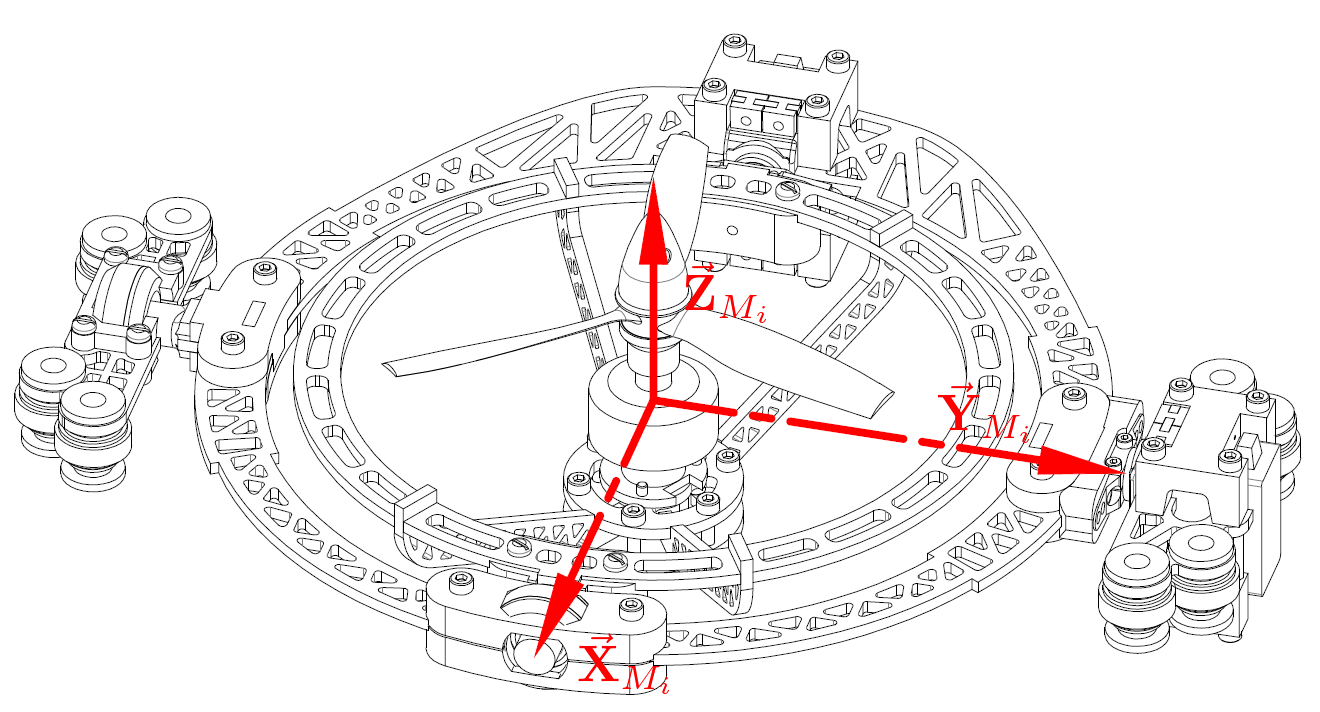
\includegraphics[width=0.8\textwidth]{figs/motor-axes}
\caption{Aligned Motor Frame Axes}
\label{fig:motor-axes}
\end{figure}
\par
The motor frames, numbered $1-4$, transform to the body frame first by an angle of $\lambda_i$ about the $\vec{X}_{M_i}$ axis. Then by $\eta_i$ about the $\vec{Y}_{M_i'}$ axis in an intermediate $M_i'$ frame. The second servo actuates $\eta_i$ to produce a second intermediate frame $M_i''$, the servo is fixed in the $M_i'$ frame. Finally there is a relative $\vec{Z}_{M_i''}$ rotation between $\mathcal{F}^b$ and $\mathcal{F}^{M_i''}$. The layout of all four motor modules are such that the $\vec{Z}$ axis transformation between the intermediate frame $\mathcal{F}^{M_i''}$ and $\mathcal{F}^b$ are all constants; $0,~90^{\circ},~180^{\circ}~\text{or}~270^{\circ}$. Each modules' state is fully described by $[\Omega_{i},~\lambda_{i},~\eta_{i}]^{T}$ for $i\in [1:4]$.
\begin{figure}[hbtp]
\centering
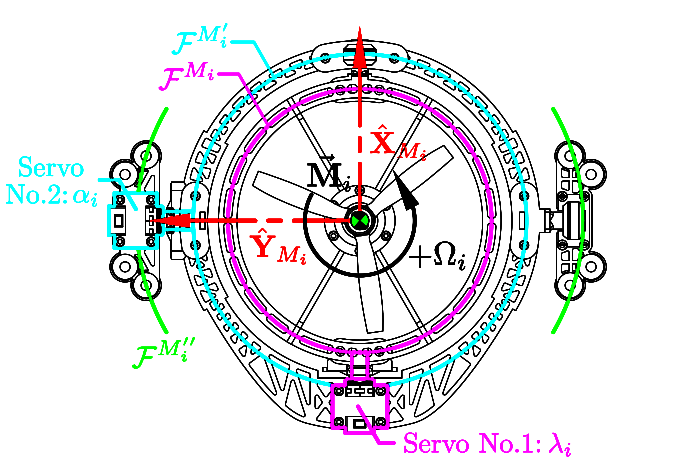
\includegraphics[width=0.6\textwidth]{figs/motor-frame}
\caption{Intermediate Motor Frames}
\label{fig:motor-frame}
\end{figure}
\par
The four motor modules are aligned relative to the body's XYZ axes as show in Fig:\ref{fig:body-frame}. Modules 1 and 3 have their X-axes respectively in the positive and negative X direction of the body frame. Similarly Modules 2 and 4 have their X-axes in the positive and negative Y directions of the body frame.
\begin{figure}[htbp]
\centering
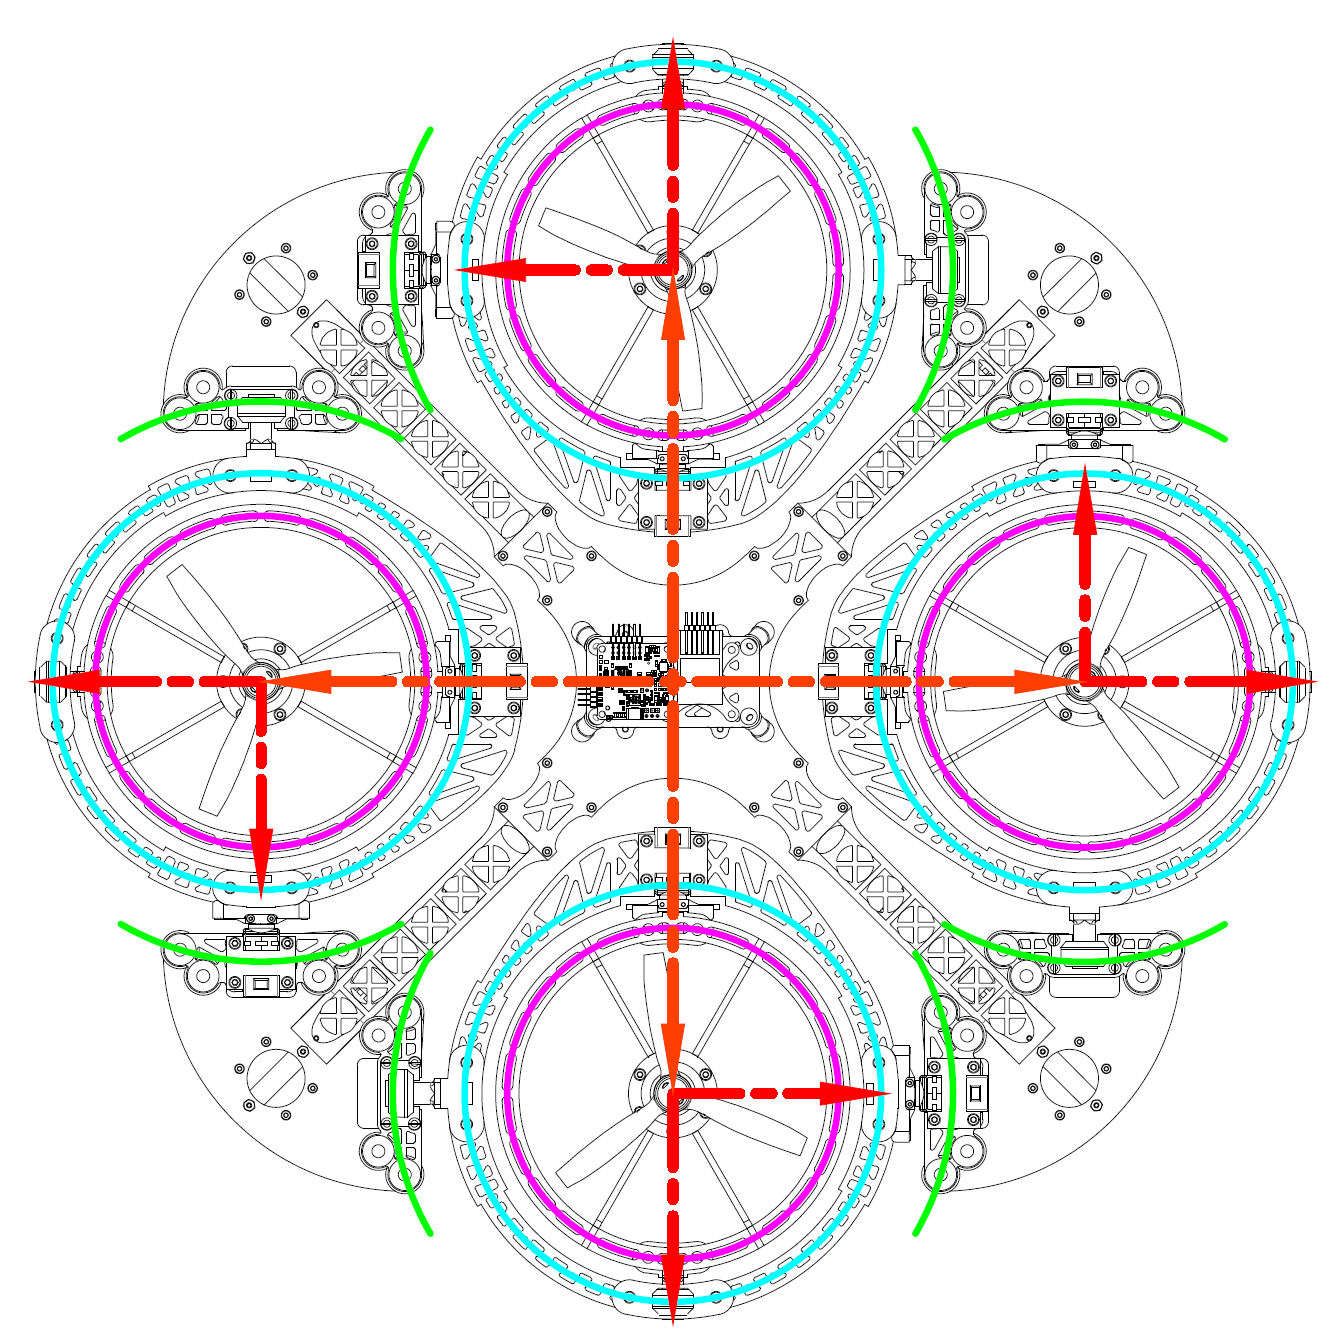
\includegraphics[width=0.8\textwidth]{figs/body-frame}
\caption{Body Frame Axes Layout}
\label{fig:body-frame}
\end{figure}
\par
Transformation relationships from each of the motor frames to the body can be characterized as:
\begin{subequations}
\begin{equation}
\vec{v}_b=\mathbb{R}_z(-\sigma_i)\mathbb{R}_y(-\eta_i)\mathbb{R}_z(-\lambda_i)\vec{v}_{M_i},~\sigma_i\in[0, 90^{\circ}, 180^{\circ}, 270^{\circ}]
\end{equation}
\vspace{-10pt}
\begin{equation}
\mathbb{R}_z=\begin{bmatrix}
1 & 0 & 0\\
0 & 1 & 0\\
0 & 0 & 1
\end{bmatrix}, \begin{bmatrix}
0 & -1 & 0\\
1 & 0 & 0\\
0 & 0 & 1
\end{bmatrix}, \begin{bmatrix}
-1 & 0 & 0\\
0 & -1 & 0\\
0 & 0 & 1
\end{bmatrix}, \begin{bmatrix}
0 & 1 & 0\\
-1 & 0 & 0\\
0 & 0 & 1
\end{bmatrix}~\text{for}~i\in[1,2,3,4]~\text{respectively}
\end{equation}
\end{subequations}
The entire actuator space, including propeller speed $\Omega_i~[rps]$, is then ($\in\mathbb{R}^{12}$)\footnote{Disambiguation: An omission of axial subscript on the $\mathbb{R}$ symbol implies a real space of the superscript dimension.}, or rather $\mathbb{U}\in\mathbb{R}^{12}$. The actuator input set $u \in \mathbb{U}$ is then structured as:
\begin{equation}
u_{\in\mathbb{U}}=\big[ \Omega_{1} ~ \lambda_{1} ~ \eta_{1} ~ \ldots ~ \Omega_{4} ~ \lambda_{4} ~ \eta_{4}  \big]^T
\end{equation}
%====================================================
\section{Design}
\label{sec:proto.design}
%====================================================
\begin{figure}[htbp]
\centering
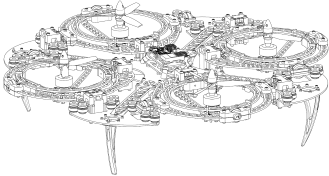
\includegraphics[width=\textwidth]{figs/iso-design}
\label{fig:iso-design}
\caption{Isometric layout of the designed prototype}
\end{figure}
The actual prototype went through a series of different design iterations, all aimed at using as many off-the-shelf RC components as possible whilst attempting to optimize construction costs. A significant factor in the design was the net weight whose upper limit, as mentioned before, is inherently linked to the thrust produced by the motors used. Some of the more important design aspects are discussed here in order to give context to some of the dynamics derived in the next chapter. The actuator suite's functionality and transfer characteristics are presented here. Finally a brief overview of the electrical systems layout is given with the components associated electrical characteristics listed. A review of the physical prototype realized and control loop implementation is detailed in Chapter:\ref{ch:flight}~along with actual flight test results.
%====================================================
\subsection{Actuation}
\label{subsec:proto.design.actuation}
%====================================================
\begin{figure}[hbtp]
\begin{subfigure}{.5\textwidth}
\centering
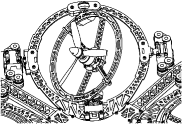
\includegraphics[width=\textwidth]{figs/motor-assembly}
\caption{Motor Module Assembly}
\label{fig:motor_assembly}
\end{subfigure}
\begin{subfigure}{.5\textwidth}
\centering
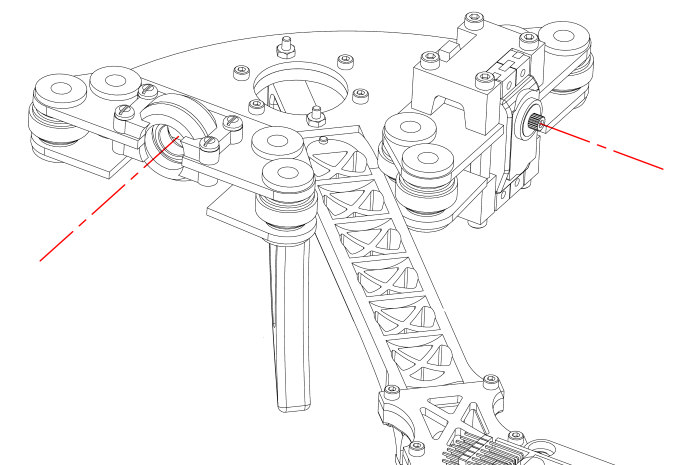
\includegraphics[width=\textwidth]{figs/motor-support}
\caption{Motor Frame Damping Support Assemblies}
\label{fig:motor_support}
\end{subfigure}
\caption{Motor Assembly}
\end{figure}
The novel component of the design is articulation of each motor module, independently redirecting the thrust generated by each lift propeller. Within each module are servos affixed onto sequential rings to pitch and roll the substructures' axes. The gyroscope-like frame which surrounds each motor/propeller pair accommodates the relative movement. Aligned with each servo is a coaxial support bearing. The coaxial bearing and actuator servos do have a mass disparity that results in a gravitational torque arm. Unfortunately, due to weight constraints, counter balance masses cannot be introduced. Consequences from the center of mass variations must either be compensated for (\emph{plant dependent solution}) or exploited in the dynamics (\emph{additional non-linear actuator plants}). The precise effects are quantified numerically next in Section:\ref{subsec:proto.design.inertia}.
\par
Each module is designed such that thrust vector produced coincides with the two rotational axes intersections (Fig:\ref{fig:motor_assembly}). There's no perpendicular displacement of generated thrust vectors relative to the body's X-Y-Z origin\footnote{Although the center of gravity does have a time varying position dependent on the 8 servos' positions}. It's more prudential to ensure intersection of the thrust vector with the rotational center than to balance the masses undergoing rotation. A thrust dependent torque arm is harder to compensate for than a gravitational torque given the complexity with modeling a propellers' aerodynamic thrust (Section:\ref{subsec:dynamics.aero.bem}).
\par
The primary frame has silicon damping balls between brackets which attach to the motor gyroscope assembly (Fig:\ref{fig:motor_support}). For damping to be effective there has to be a equatable relative masses between the two bodies to be damped. A smaller damping assembly in the center of the frame houses all the electronics and power distribution circuitry. All the mounting brackets which affix the motor moduels are 3D printed from CAD models using an Ultimaker V2+\cite{ultimaker}. There is a complete bill of materials for all parts used, including working drawings for each 3D printed bracket and the laser cut frame, in Appendix:\ref{app:bom}.
\par
\begin{figure}[hbtp]
\centering
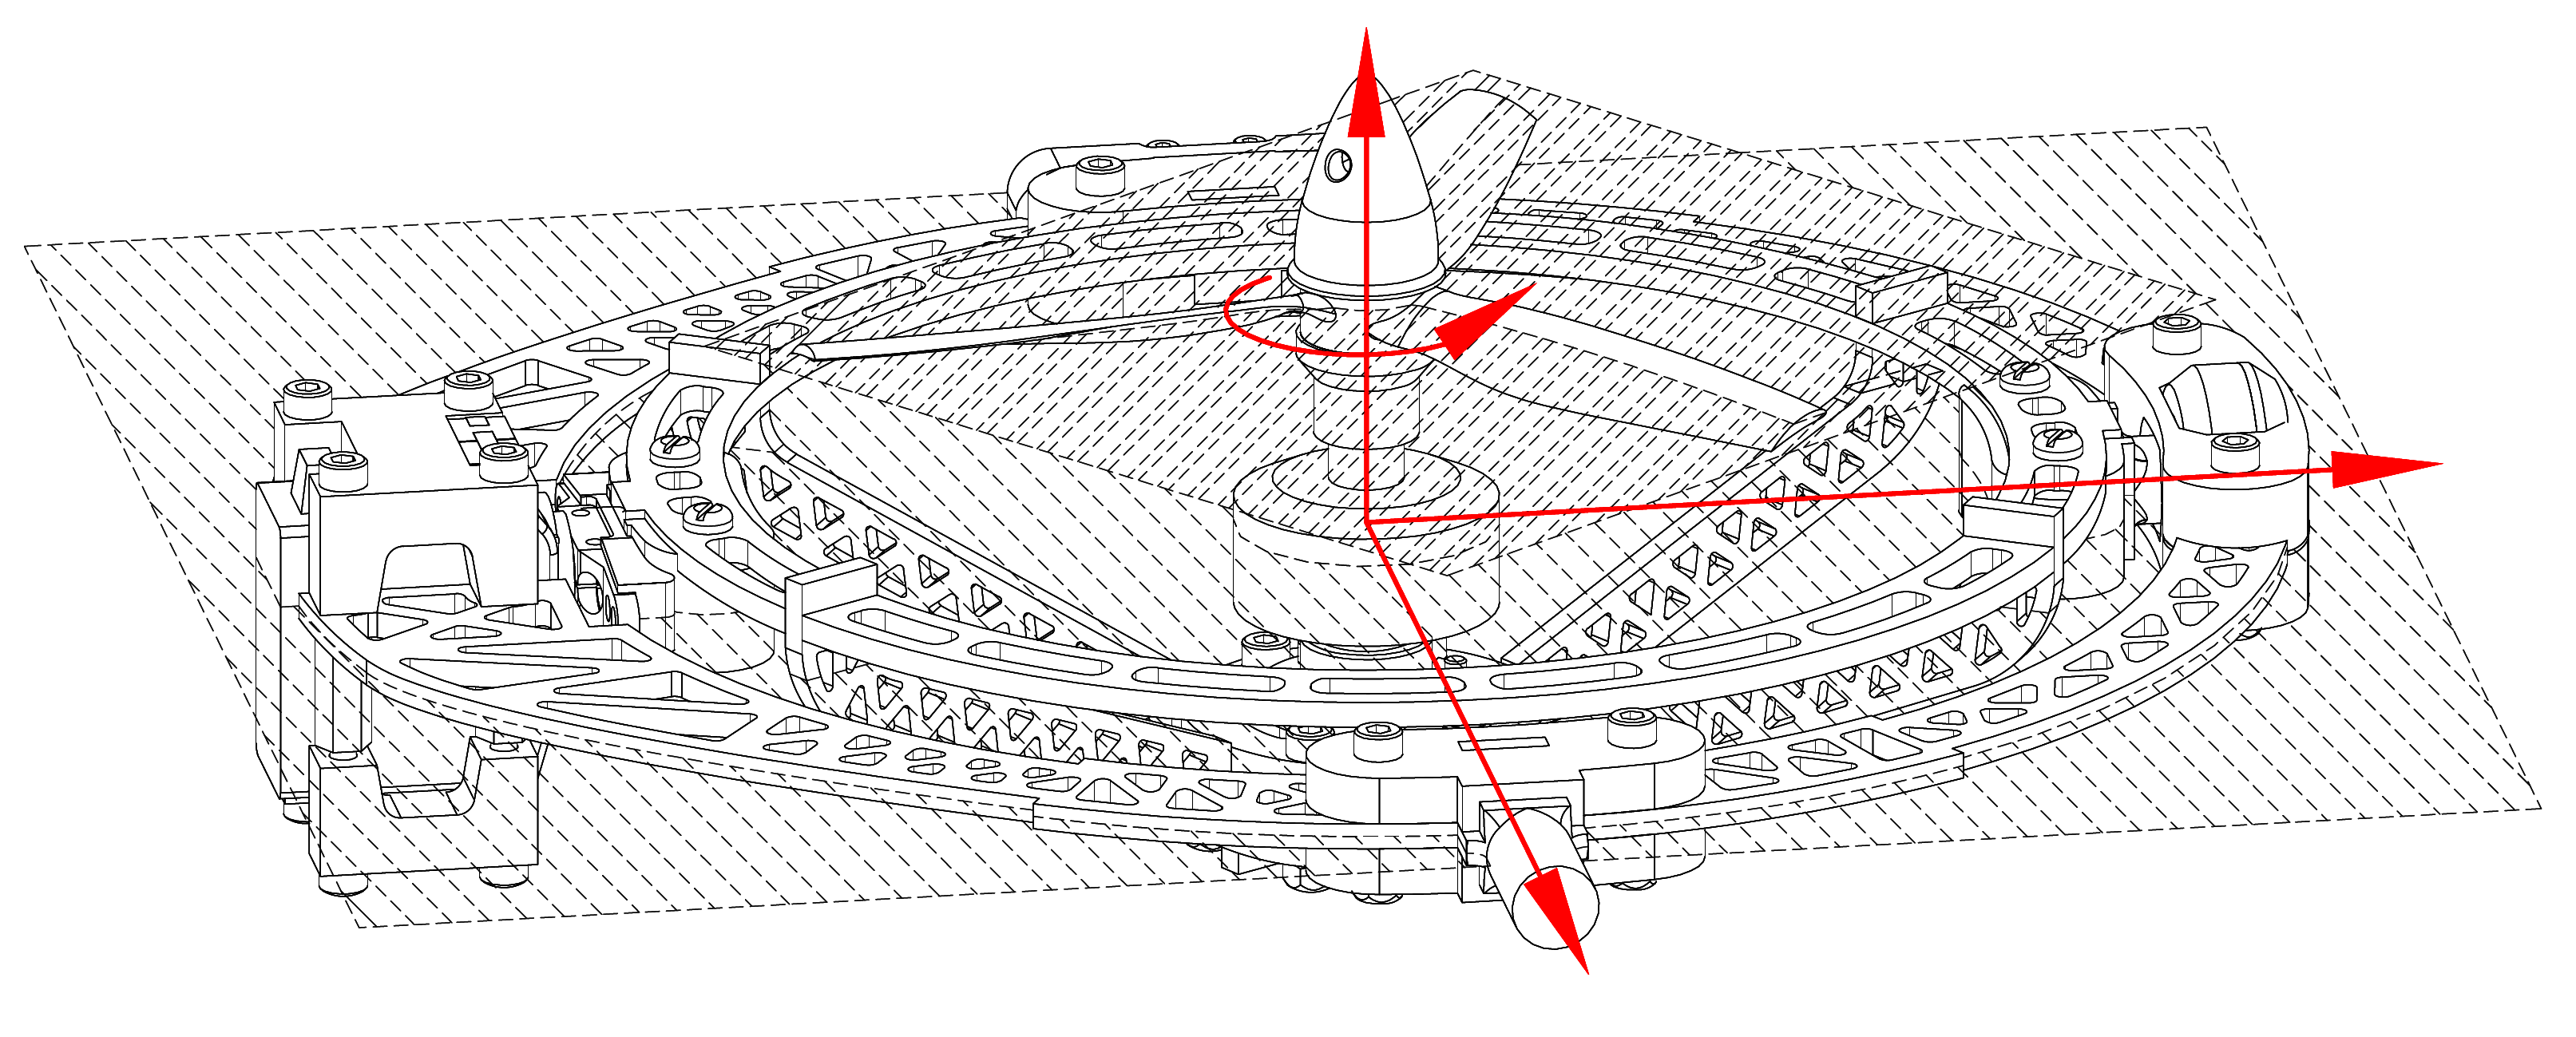
\includegraphics[width=\textwidth]{figs/motor-prop}
\caption{Difference between propeller and motor planes}
\label{fig:motor_prop}
\end{figure}
The propellers rotational plane is not exactly the aligned with the plane made by the $\vec{X}_{M_i}$ and $\vec{Y}_{M_i}$ rotational servo axes (Fig:\ref{fig:motor_prop}). The offset is approximately 28.2 mm and must be considered when evaluating pitch/roll gyroscopic torque responses later in Section:\ref{subsec:dynamics.nonlinearities.gyrotorques}. The propellers are 6 inch ($6 \times 4$) 3-Blade plastic Gemfam propellers, powered Turnigy DST-700KV Outrunner Brushless DC motors. The thrust produced as a funciton of angular velocity (in RPS) for the propellers is derived in Section:\ref{subsec:dynamics.aero.bem}. The BLDC motors are controlled with Hobbywing XRotor 15A ESC modules with an inline Orange RPM Sensor. The transfer function for the combined unit is presented subsequently in Section:\ref{subsec:proto.design.transfer}. Power for the quadrotor is supplied not from a battery bank but from a power tether. Tethered power will ensure consistent flight time and reduces the concern of payload strain on the available lift actuation. Power lines to both the BLDC motors and servos are both supplied conventionally, however an ideal construction would see slip-rings for each module's supply. Power transmission lines are affixed such that they don't impede rotation. 
\begin{figure}[htbp]
\centering
\begin{subfigure}{0.49\textwidth}
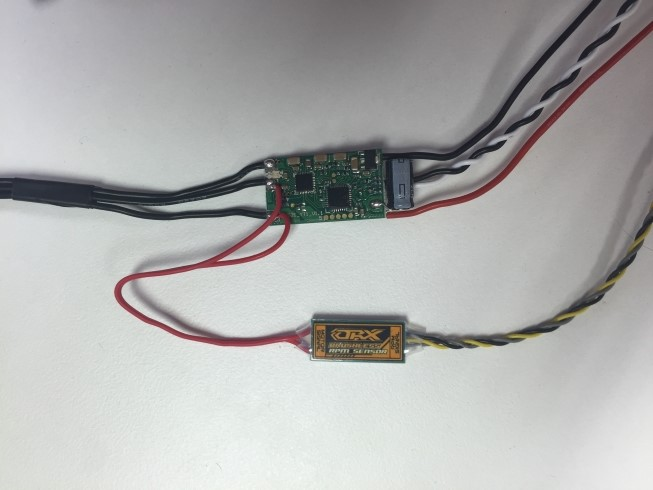
\includegraphics[width=\textwidth]{figs/motor-esc}
\caption{BLDC ESC \& RPM Sensor Assembly}
\label{fig:bldc-esc}
\end{subfigure}
\begin{subfigure}{0.49\textwidth}
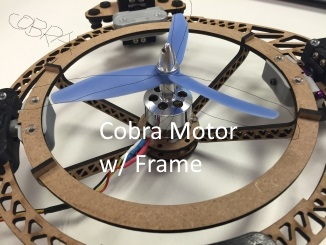
\includegraphics[width=\textwidth]{figs/motor-bldc}
\caption{Turnigy DST-700KV BLDC Motor}
\label{fig:bldc-motor}
\end{subfigure}
\end{figure}
\par
Metal gear Corona DS-339MG digital servos are used for the two axes of rotation (Fig:\ref{fig:motor-servo}). Each servo has a range of $180^{\circ}$, positioned such that a $\text{zero}^{\text{th}}$ offset aligns the motor modules  adjacent to the body frame and has a $\pm 90^{\circ}$ range. A digital servo updates at 330 Hz, faster than a 50 Hz analogue servo equivalent (Table:\ref{tab:servo}). This means the otherwise $20$ms zero-order analogue sampling becomes a less significant $3.30$ms zero-order holding time. Both the $\vec{X}_{M_i}$ and $\vec{Y}_{M_i}$ axis servos will be rotating a large loading mass and so their \emph{open loop} plant dynamics are determined empirically in Section:\ref{subsec:proto.design.transfer} using test data included in Appendix:\ref{app:systemdat}.
\begin{table}[h]
\centering
\fbox{
\begin{minipage}{0.7\textwidth}
\begin{tikztimingtable}
50 Hz: &[C] 31{C} G\\
Analogue Servo &1{L} 1.5{H} 18.5{L} 1.5{H} 10{L}\\
Digital Servo&1{L} 15{1.5{H} 1.53{L}}\\
\end{tikztimingtable}
\end{minipage}
}
\caption{Analogue \& Digital Timing Signals}
\label{tab:servo}
\end{table}
\begin{figure}[htbp]
\centering
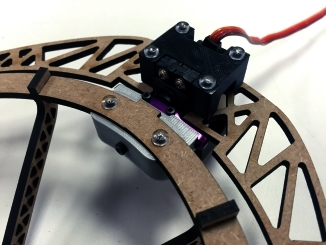
\includegraphics[width=0.5\textwidth]{figs/motor-servo}
\caption{Corona Servo Bracket}
\label{fig:motor-servo}
\end{figure}
%====================================================
\subsection{Inertial Matrices \& Mass}
\label{subsec:proto.design.inertia}
%====================================================
An undesirable side effect of the added rotations are the inertial responses produced from such rotations. Given Newtons' Second Law of rotational motion, the induced rotations are going to produce an equal but opposite reaction onto the principle inducing frame. Similarly a gyroscopic cross product from rotational velocities is also present. Such first and second order effects are mostly negligible, angular rates are usually small enough to approximate as zero, $\omega_b\approx\vec{0}$. A dynamic set-point (non-zero) attitude tracking plant is however going to produce sizeable time varying body angular velocities and accelerations so, unlike a standard quadrotor, such effects have to be accounted for.
\begin{figure}[htbp]
\centering
\begin{subfigure}{0.49\textwidth}
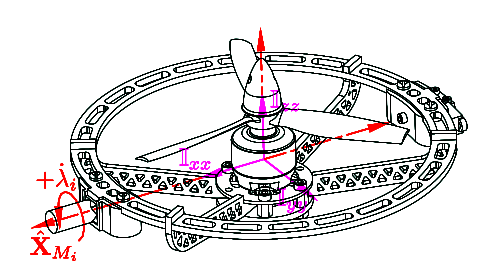
\includegraphics[width=\textwidth]{figs/inertia-inner}
\caption{Inner Ring Rotational Structure}
\label{fig:inertia-inner}
\end{subfigure}
\begin{subfigure}{0.49\textwidth}
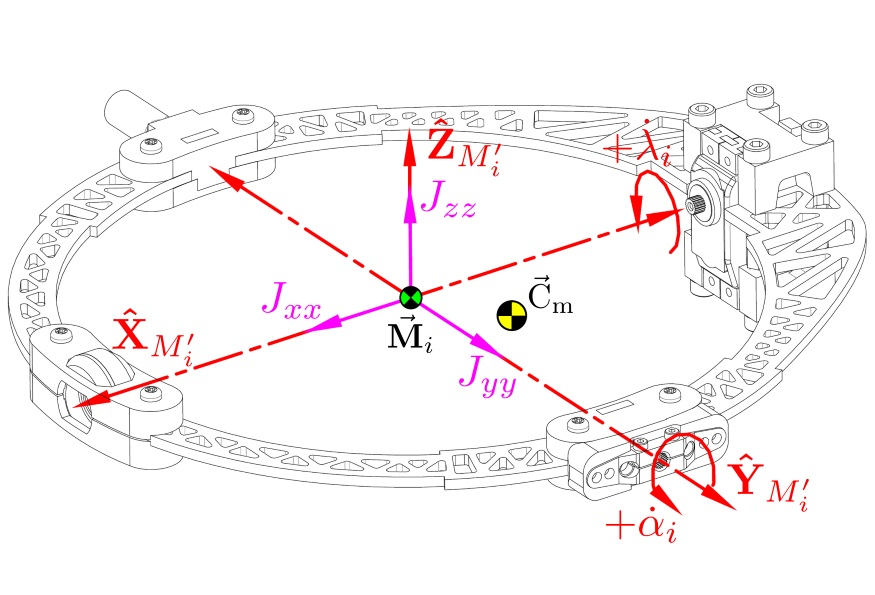
\includegraphics[width=\textwidth]{figs/inertia-middle}
\caption{Middle Ring Rotational Structure}
\label{fig:inertia-middle}
\end{subfigure}
\caption{Inertial Measurement References}
\end{figure}
\par
The manifestation of the aforementioned torque responses are explored in thorough detail in Section:\ref{sec:dynamics.nonlinearities}. Both of those effects are dependent on the rotational body's moment of inertia\footnote{All inertias calculated in Solidworks with overridden mass properties} about its respective rotational axis. The magnitude of the inertia is obviously a byproduct of the structures' design. Starting with the innermost assembly, in each Motor Frame $\mathcal{F}^{M_i}$, the inner most ring structure (Fig:\ref{fig:inertia-inner}) is a 99g assembly (all parts included). The rotational center is also the center its of mass, rotated by $\lambda_i^{~\circ}$ about its $\vec{X}_{M_i}$ axis. The inner rings' moment of inertia (centered as in Fig:\ref{fig:inertia-inner}) is found to be:
\begin{subequations}
\begin{equation} \label{eq:inertia.inner.a}
\mathbb{I}_{M_i}=\begin{bmatrix}
588.841 & -0.276 & 0.249\\
-0.276 & 1966.600 & 0.897\\
0.249 & 0.897 & 2141.779\\
\end{bmatrix}~~[g.cm^2]
\end{equation}
\vspace{-5pt}
\begin{equation} \label{eq:inertia.inner.b}
\approx diag\big(588.84 ~1966.60 ~2141.78\big)\times10^{-7}~~[kg.m^2]
\end{equation}
\end{subequations}
The effect of a rotating propeller on the moment of inertia can be approximated by a solid disc and hence the inner rings' moment of inertia is regarded as consistent and symmetrical. The inertial tensor about that $\vec{X}_{M_i}$ axis is then $\mathbb{I}_{\lambda}=588.8\times10^{-7} [kg.m^2]$.
\par
The second $\lambda_i$ actuating servo and bearing supports are affixed to the intermediate middle ring assembly (Fig:\ref{fig:inertia-middle}). The middle ring frame, $\mathcal{F}^{M_i~'}$, is a 102g structure, excluding the inner most ring. Collectively it's 201g for both the inner and middle rings structures. That middle ring is then rotated by $\eta_i^{~\circ}$ about its $\vec{Y}_{M_i}$ axis. The compound body's inertia about its axis of rotation, $\vec{Y}_{M_i}$, is a combination of both the middle rings' inertia and the inner ring.  The latter's contribution being a function of the rotation angle $\lambda_i^{~\circ}$ which, from the conservation of angular momentum theory \cite{inertiatensor}\footnote{$\mathbb{R}_x$ is a full rank and square, so an inverse $\mathbb{R}_x~^{-1}$ always exists}, is:
\begin{subequations}
\begin{equation}\label{eq:inertia.middle.a}
\mathbb{I}_{M_i~'}=\mathbb{I}_{middle}+\mathbb{R}_x(\lambda_i)\big(\mathbb{I}_{inner}\big)\mathbb{R}_x(\lambda_i)^{-1}
\end{equation}
\begin{equation} \label{eq:inertia.middle.b}
\text{If} ~~\mathbb{I}_{middle}=\begin{bmatrix}
3024.303 & -0.395 & 406.870\\
-0.395 & 8791.879 & -0.013\\
406.870 & -0.013 & 11580.579\\
\end{bmatrix}~~[g.cm^2]
\end{equation}
\begin{equation} \label{eq:inertia.middle.c}
\rightarrow\begin{bmatrix}
588.851 & -0.276 & 0.248\\
-0.276 & 1966.602 & 0.897\\
0.248 & 0.897 & 2129.127\\
\end{bmatrix}
\end{equation}
\end{subequations}
With $\mathbb{I}_{inner}=\mathbb{I}_{M_i}$ being the inertia from Eq:\ref{eq:inertia.inner.a} which is rotated by $\mathbb{R}_x(\lambda_i)$. The complete inertia, as a function of rotation angle, is then Eq:\ref{eq:inertia.middle.c}. This is the first of many non-trivial aspects to this aircrafts' design which require a heavily plant dependent control solution. 


The mass of the co-axial servo and bearing are not balanced so the structures' centre of mass is not at its rotational centre. 

 The next sequential ring rotates
%====================================================
\subsection{Actuator Transfer Functions}
\label{subsec:proto.design.transfer}
%====================================================

%====================================================
\subsection{Overall Aspects}
\label{subsec:proto.design.aspects}
%====================================================
\subsubsection{Vibration Damping}
%====================================================
\subsubsection{Landing Skids}
%====================================================
\subsubsection{Motors \& ESCs}
%====================================================

%====================================================
\section{System Layout}
\label{sec:proto.layout}
%====================================================
\subsection{Electrical Design}
\subsection{Component Characteristics}